In order to evaluate the proposed solutions to the task allocation problem among UAVs, a simulation was implemented in NetLogo\citep{tisue2004netlogo} (version 5.3.1). The tasks and \uavs\ are represented by specific symbols.
Figure \ref{fig:simulacao} illustrates the simulation graphical interface, where the symbol for the tasks is represented by a ``X'' shape and the symbol for a \uav\ has the shape of an airplane.

\begin{figure}[h!]
	\begin{center}
		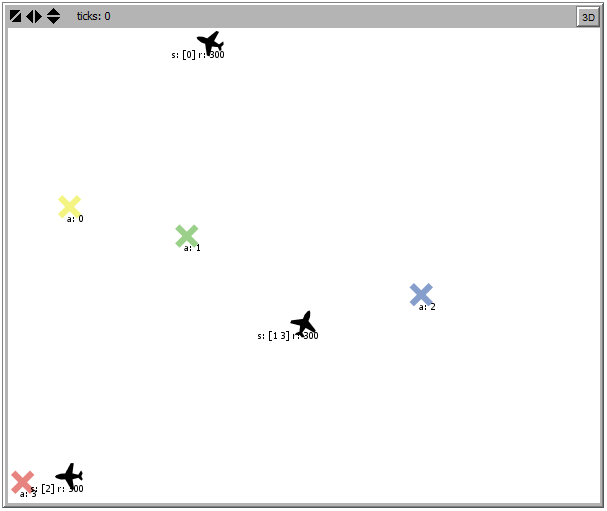
\includegraphics[scale=0.50]{simulation.png}
		\caption{Simulation in the NetLogo}
		\label{fig:simulacao}
	\end{center}
\end{figure}

According to problem formulation (Section \ref{sec:problem}), each task has its location $\langle x,y \rangle$, an associated type of target and the amount of resource required for its execution. The difference in the colors of the tasks represents the different types of targets in Figure \ref{fig:simulacao}, for example, the color red may represent a fire places and the color blue a train of parked vehicles. Each UAV, in addition to its location $\langle x,y \rangle$ and its sensor list, has a ``to-do'' list of tasks. This list starts empty, and when the \uav\ selects a task, it adds the task to this list. 
The ``to-do'' list is a FIFO: the first selected task is the first one to be performed.

The simulation was implemented so that at each tick (simulation time progression unity), all UAVs move one pixel. 
The ticks are used as makespan (total time that elapses from the beginning to the end of the execution). It will never exceed the mission deadline. The execution ends when the \uavs\ complete all tasks they have selected to perform.
It is noteworthy that the makespan (elapsed time) may be easily converted into traveled distance by each UAV since all UAVs move one pixel per tick.

Only one token is released to the \uavs. The token contains the mission tasks and a list of visited agents. This list starts empty and each \uav\ that receives the token adds its ID in the list. At each tick, the token is sent to a random \uav\ that has not yet received the token in the current round, i.e. a \uav\ that is not in the list of visited agents. The token also has a list of unavailable agents. This list is used by the proposed algorithms AL, SAL and LAL (see Section \ref{sec:al}).
When a UAV receives the token, it runs the algorithm to choose the tasks it will perform. 

Several experimental scenarios were created in order to analyze different situations. The scenarios vary in amount of mission tasks, number of agents and size of the area (in pixels) in which they are situated, as listed in the following:

\begin{enumerate}
	\item 3 \uavs; 4 tasks; 300 ticks as deadline; 100 x 80 px area size. \label{case:4tasks}
	\item 3 \uavs; 8 tasks; 300 ticks as deadline; 100 x 80 px area size. \label{case:8tasks}
	\item 3 \uavs; 16 tasks; 300 ticks as deadline; 100 x 80 px area size. \label{case:16tasks}
	\item 3 \uavs; 32 tasks; 300 ticks as deadline; 100 x 80 px area size. \label{case:32tasks}
	\item 6 \uavs; 64 tasks; 300 ticks as deadline; 200 x 160 px area size. \label{case:64tasks}
	\item 9 \uavs; 96 tasks; 300 ticks as deadline; 300 x 240 px area size. \label{case:96tasks}
\end{enumerate}

Each set of \uavs\ -- with 3, 6, and 9 \uavs\ -- were randomly created once. For example, the set of 3 \uavs\ were created once and used in scenarios \ref{case:4tasks}, \ref{case:8tasks}, \ref{case:16tasks}, \ref{case:32tasks}. 
The \uavs' location $\langle x,y \rangle$ were defined randomly, respecting the limit of the scenario's area.
The number of sensors that each \uav\ was equipped as well as the types of sensors were also assigned with random values. Each \uav\ was equipped with one or two sensors of types $s_0$, $s_1$, $s_2$ or $s_3$.

The same was applied for the tasks. The tasks location $\langle x,y \rangle$ and the type of target were defined randomly. 
Each task was assigned a single type of target, which may be of the types $a_0$, $a_1$, $a_2$ or $a_3$.
Only the amount of resources needed to execute a task ($c_j$) was fixed at ten time units (ticks) for all tasks. 

Table \ref{table:quality} presents the sensors' quality to detect each type of target. These values were used in all scenarios. According to this configuration, the target $a_0$, for example, can be detected by the sensors $s_0$ and $s_2$, but with different qualities, while sensors $s_1$ and $s_3$ are unable to detect $a_0$.

\begin{table}[h!]
	\small
	\fontsize{8}{8}\selectfont
	\centering
	\caption{Quality of each sensor to detect the different types of target}
	\label{table:quality}
	\begin{tabular}{|l|c|c|c|c|} \hline
		Sensor / target  & $a_0$  & $a_1$  & $a_2$  & $a_3$    \\ \hline
		$s_0$              & $1.0$  & $0$  & $0.3$  & $0.5$      \\ \hline
		$s_1$              & $0$  & $0$  & $1.0$  & $0$           \\ \hline
		$s_2$              & $0.2$  & $0$  & $0$  & $1.0$        \\ \hline
		$s_3$              & $0$  & $1.0$  & $0$  & $0.3$        \\ \hline
	\end{tabular}
\end{table}


The scenarios were run 30 times for each proposed algorithm. 
In all experiments, the UAVs' capabilities were computed using Equation \ref{eq:capability} with $\alpha = 0.6$, giving higher importance to the distance factor.
Different stimulus values were also tested, but only results with the value 0.6 are shown, as this value presented better results in most cases, as it is known for the Swarm-GAP \citep{ferreira2010robocup}.

The experiments were conducted in a PC with 1.70GHz, 4GB of RAM and SO Windows 8.1 Pro 64 bits. 
The results obtained using the proposed solutions as well as Swarm-GAP are presented and discussed in next section.

